\documentclass[12pt]{article}

\usepackage{mathtools, amssymb, amsmath}
\usepackage{enumitem}
\usepackage[margin=2.5cm]{geometry}
\usepackage{setspace}
\usepackage{graphicx}
\graphicspath{ {./images/} }

\renewcommand{\baselinestretch}{1.5}
\everymath{\displaystyle}

\begin{document}
	\section*{Q1}
	\begin{enumerate}[label=\alph*)]
		\item 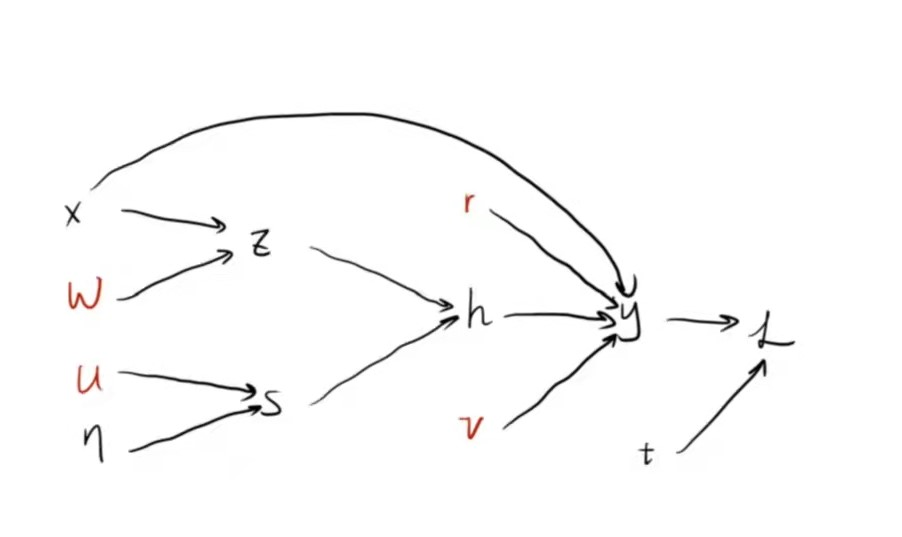
\includegraphics[scale=0.4]{1a}
		\item \begin{align*}
			\overline{y}&=y-t\\
			\overline{\textbf{v}}&=\overline{y}\textbf{h}^T\\
			\overline{\textbf{r}}&=\overline{y}\textbf{x}^T\\
			\overline{\textbf{h}}&=\overline{y}\textbf{v}^T\\
			\overline{\textbf{z}}&=\overline{\textbf{h}}\sigma(\textbf{s})\\
			\overline{\textbf{s}}&=\overline{\textbf{h}}(z\odot\sigma'(\textbf{s}))\\
			\overline{\textbf{W}}&=\overline{\textbf{z}}\textbf{x}\\
			\overline{\textbf{U}}&=\overline{\textbf{s}}\eta\\
			\overline{\eta}&=\overline{\textbf{s}}\textbf{U}\\
			\overline{\textbf{x}}&=\overline{\textbf{z}}\textbf{W}+\overline{\textbf{y}}\textbf{r}^T
		\end{align*}
	\end{enumerate}
	\newpage
	
	\section*{Q2}
	\begin{enumerate}[label=\alph*)]
		\item For each $x$, write \[p(x,t|\theta,\pi)=\prod^9_{i=0}[\pi_i^{t_i}
		\prod^{784}_{j=1}(\theta_{ji})^{x_j}(1-\theta_{ji})^{(1-x_j)}]\]
		Assume $\{x_1,\cdots,x_N\}$ are all the $N$ samples, let $x_{Nj},t_{Nj}$ be the $x_j,t_j$ value of the $N$th sample, the likelihood function is:
		\[L(\theta,\pi)=\prod_{k=1}^{N}\prod^9_{i=0}[\pi_i^{t_{ki}}
		\prod^{784}_{j=1}(\theta_{ji})^{x_{kj}}(1-\theta_{ji})^{(1-x_{kj})}]\]
		Take logarithm:
		\[l(\theta,\pi)=\sum^N_{k=1}\sum^9_{i=0}[t_{ki}log(\pi_i)+\sum^{784}_{j=1}x_{kj}log(\theta_{ji})+(1-x_{kj})log(1-\theta_{ji})]\]
		To find MLE of $\theta$, take derivative w.r.t $\theta_{ji}$ and set to $0$, we get\[
			\sum^N_{k=1}t_{ki}(\frac{x_{kj}}{\theta_{ji}}-\frac{1-x_{kj}}{1-\theta_{ji}})=0
		\]
		Multiply both side by $\theta(1-\theta)$, simplify we get
		\[\hat{\theta}_{ji}=\frac{\sum^N_{k=1}t_{ki}x_{kj}}{\sum^N_{k=1}t_{ki}}\]
		To find MLE of $\pi$, first write $l(\theta,\pi)=\sum^N_{k=1}(\sum^8_{i=0}t_{ki}log(\pi_i)+t_{k9}log(1-\sum^8_{i=0}\pi_i)+\cdots)$, take derivative w.r.t $\pi_i$ and set to $0$:
		\[\sum^N_{k=1}(\frac{t_{ki}}{\pi_i}-\frac{t_{k9}}{1-\sum^8_{i=0}\pi_i})=0\]
		Multiply both sides by $\pi_i(1-\pi_9)$, simplify we get
		\[\frac{\pi_i}{\pi_9}=\frac{\sum^N_{k=1}t_{ki}}{\sum^N_{k=1}t_{k9}}\]
		Sum up the functions for $10$ values of $i$s, note sum of all $\pi_i$ is $1$, and sum of $t_{ki}$ over all $k$ and $i$ is $N$, so we get
		\[\frac{1}{\pi_9}=\frac{N}{\sum^N_{k=1}t_{k9}}\]
		Do this manipulation over all values of $i$, we get MLE of $\pi_i$
		\[\hat{\pi}_i=\frac{\sum^N_{k=1}t_{ki}}{N}\]
		\item We can write
		\begin{align*}
			\log(p(t|x,\theta,\pi))&=\log(\frac{p(x,t|\theta,\pi)}{p(x|\theta,\pi)})\\
			&=\log(\frac{p(t|\pi)\prod^{784}_{j=1}(x_j|t,\theta)}{\sum^9_{i=0}p(t_i|\pi)\prod^{784}_{j=1}(x_j|t,\theta)})\\
			&=\log(\pi_c)+\sum^{784}_{j=1}(x_j\log(\theta_{jc})+(1-x_j)\log(1-\theta_{jc}))\\
			&-\log(\sum^9_{i=0}\pi_i\prod^{784}_{j=1}\theta_{ji}^{x_j}(1-\theta_{ji})^{1-x_j})
		\end{align*}
		\item The average log-likelihood is nan, because at some point the log is taken over $0$ maximum likelihood, which results in infinity error.
		\item MLE estimator plot: \\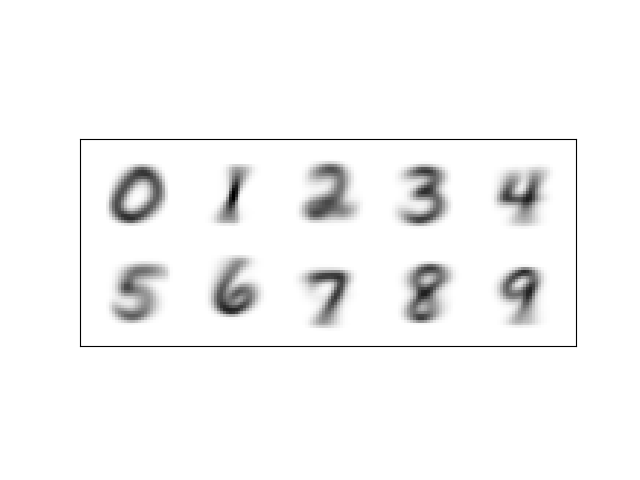
\includegraphics[scale=0.5]{mle.png}
		\item MAP estimator:\\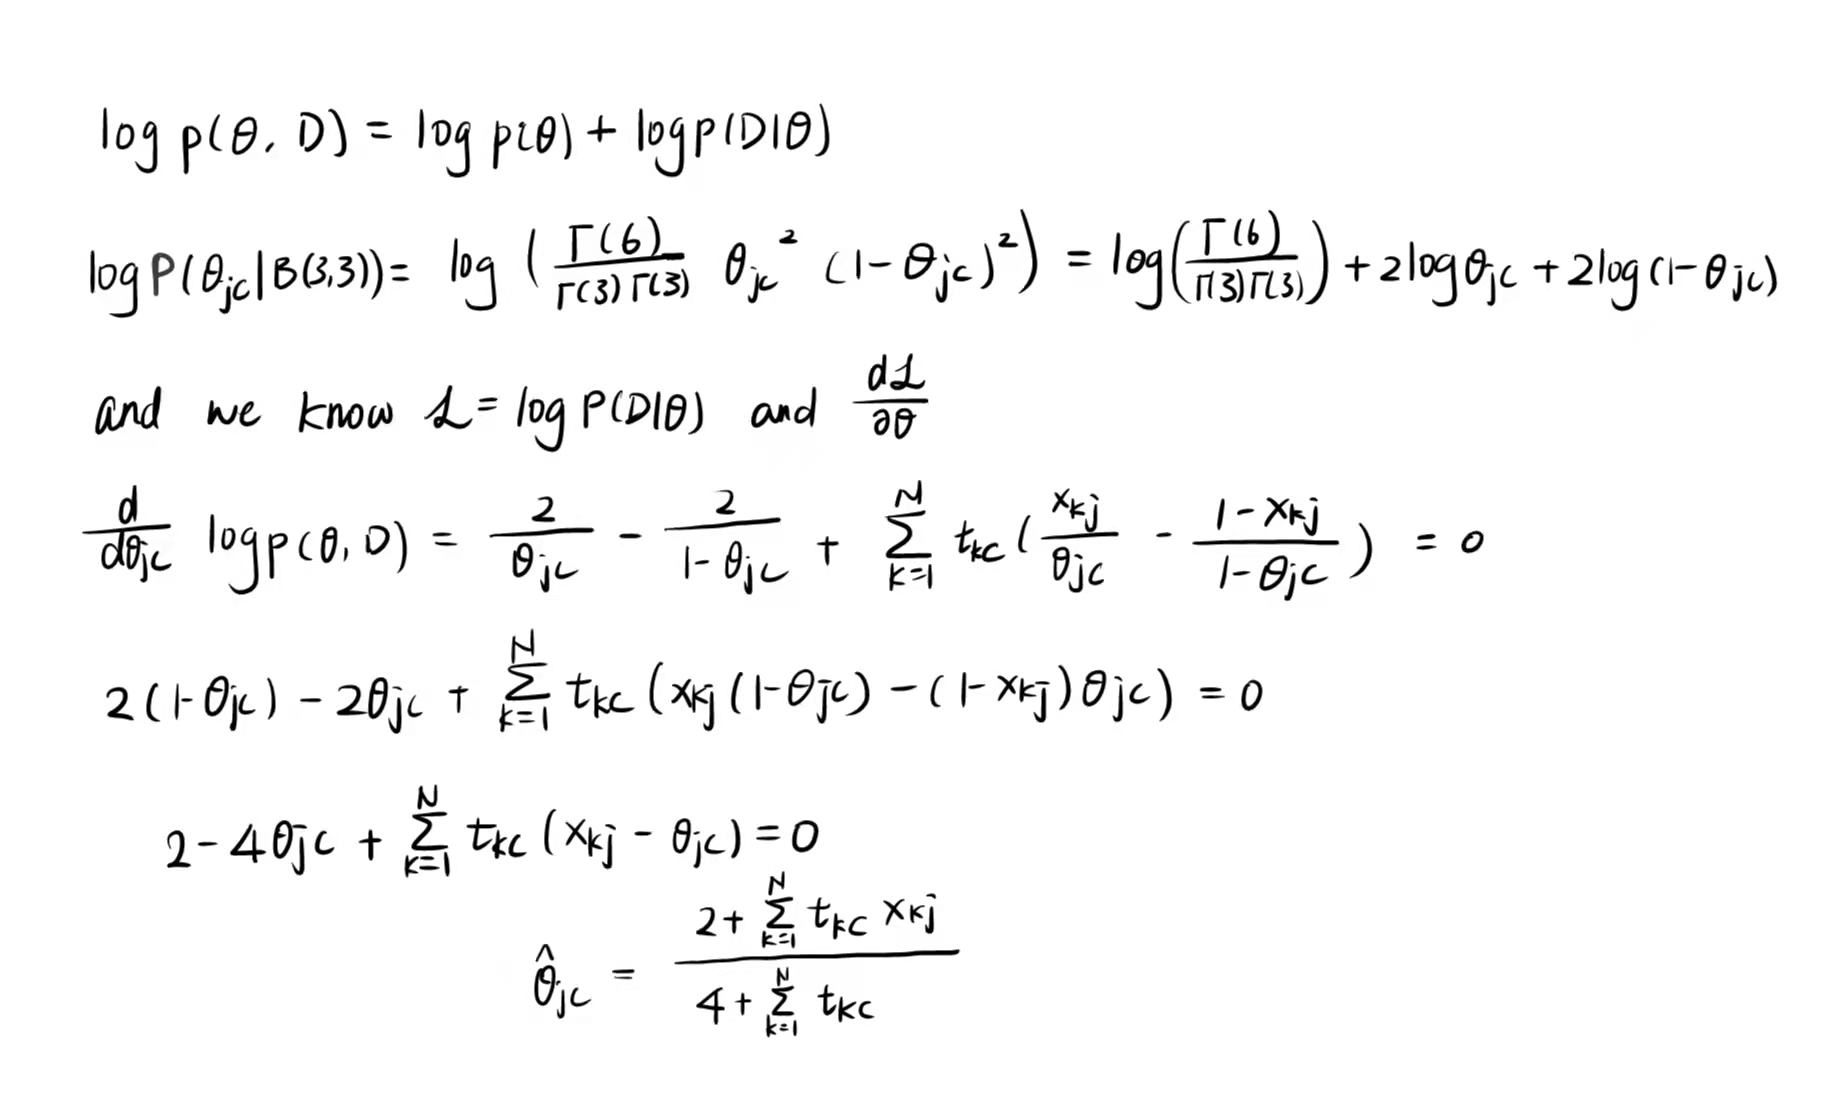
\includegraphics[scale=0.2]{2e}
		\item Average log-likelihood for MAP is -3.357\\
		Training accuracy for MAP is 0.835\\
		Test accuracy for MAP is 0.816\\
		\item MAP estimator plot: \\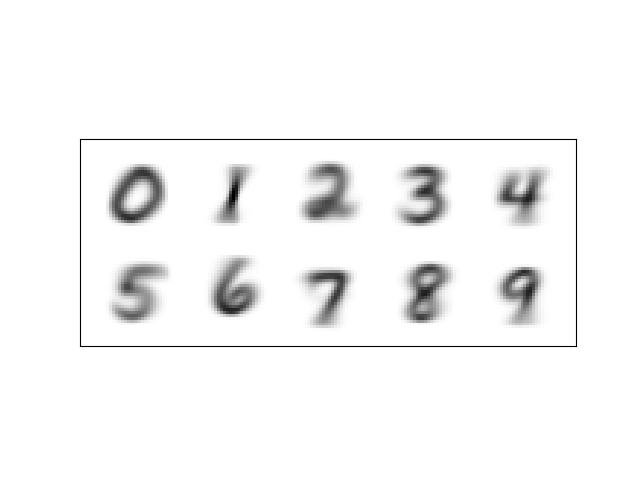
\includegraphics[scale=0.5]{map.png}
	\end{enumerate}
	
	\newpage
	\section*{Q3}
	a)\\ 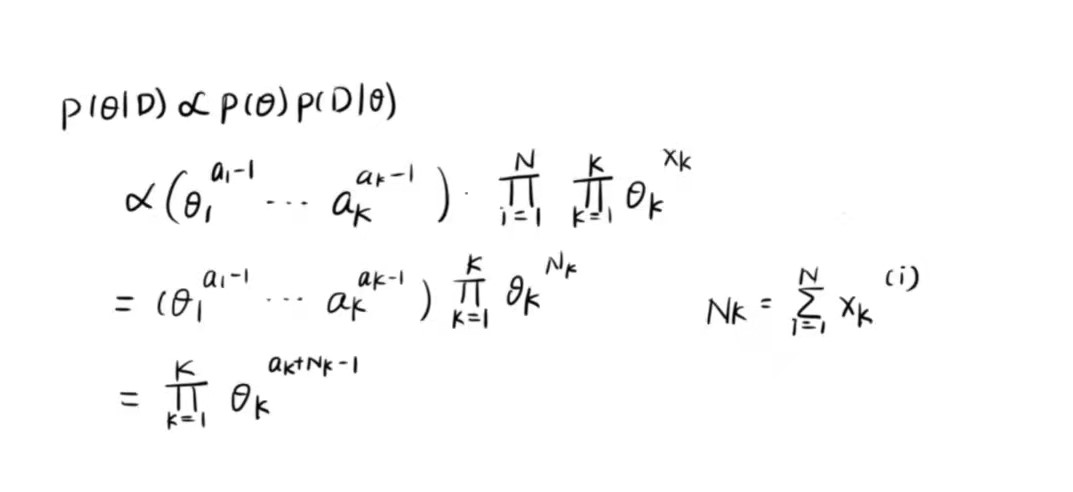
\includegraphics[scale=0.4]{3a.jpg}\\
	b)\\ 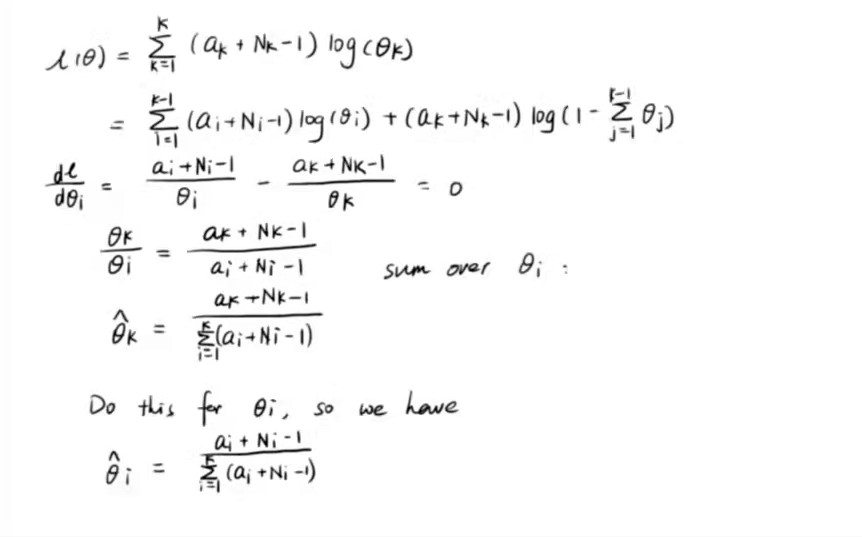
\includegraphics[scale=0.6]{3b.jpg}\\
	c)\\ 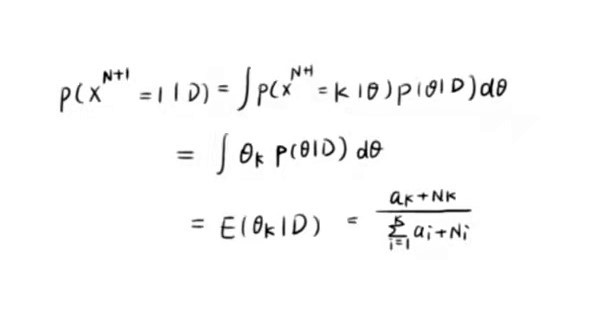
\includegraphics[scale=0.5]{3c.jpg}

\end{document}










